\section{Zoom}

El filtro LinearZoom consiste en interpolar linealmente los pixeles de la imagen, duplicando su ancho y su alto, es decir aumentando su tamaño efectivo en 4.

La interpolación lineal de los pixeles consiste en calcular los promedios de cada componente entre los pixeles adyacentes al nuevo pixel interpolado. La misma se puede representar con la siguente matriz:

\begin{table}[H]
\centering
  \begin{tabular}{ | c | c | }
    \hline
    A & B \\ \hline
    C & D \\
    \hline
  \end{tabular}
{\LARGE$\xrightarrow{LinearZoom}$}
  \begin{tabular}{ | c | c | c | c |}
    \hline
    A & (A+B)/2 & B & $\cdots$ \\ \hline
    (A+C)/2 & (A+B+C+D) & (B+D)/2 & $\cdots$ \\ \hline
    C & (C+D)/2 & D & $\cdots$ \\ \hline
    $\vdots$ & $\vdots$ & $\vdots$ & $\ddots$ \\
    \hline
  \end{tabular}
\end{table}

En el caso de la última fila y la última columna, como no existe información para interpolar, los elementos deben ser duplicados.

El filtro en sí no presenta un efecto visual muy notorio, pero el tamaño de la imagen crece.

\subsection{Implementación}

La implementación de este algoritmo requirió un enfoque distinto al que tomamos con los demás: ya que la ultima fila debe copiarse hacia abajo, nos resultó más facil recorrer la imagen de arriba hacia abajo, es decir, de los valores más altos de la matriz de pixeles. Se hace esta salvedad por el hecho que el formato proporcionado de imagen guarda las filas de inferior a superior. En los otros algoritmos esta distinción no se hizo ya que no fue necesaria.

En la implementación con SIMD, podemos aprovechar las operaciones vectoriales para operar no solo sobre las múltiples componentes a la ves, sino también sobre más de un pixel (como son sumas de hasta 4 bytes, solo requerimos tamaño word por componente).


\begin{center}

\xmm{3} \xmmQuadWord{A}{B} \\

\xmm{4} \xmmQuadWord{C}{D} \\

\texttt{PADDW} \xmm{3}, \xmm{4} \hfill

\xmm{3} \xmmQuadWord{A+C}{B+D} \\

\texttt{PSRLW} \xmm{3}, 1 \hfill

\xmm{3} \xmmQuadWord{(A+C)/2}{(B+D)/2} \\

\end{center}

\subsection{Análisis preeliminar}
\subsubsection*{Comparación de rendimiento de ASM vs C}

Dado que la interpolación lineal es un procesamiento muy conocido de imágenes, nos esperabamos que fuese uno de los filtros más beneficiados por la vectorización de los cálculos.

\begin{center}
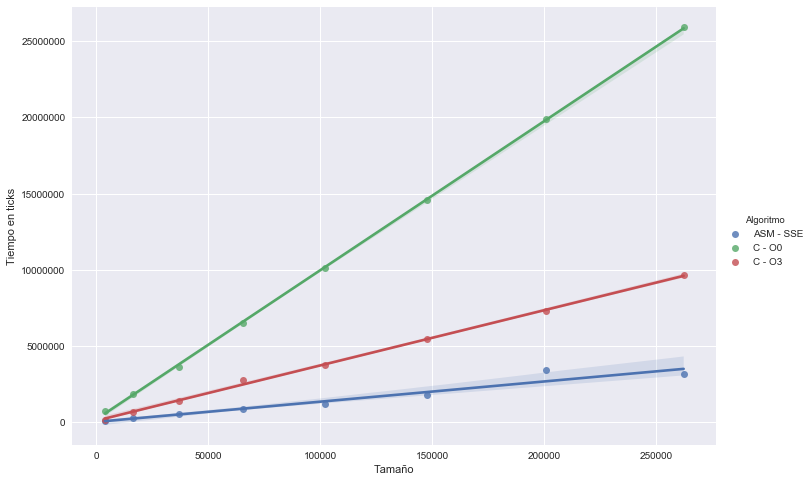
\includegraphics[scale=0.5]{img/linearZoom_CvsASMvsO3.png}
\end{center}

Efectivamente, nuestros análisis dieron que incluso con las optimizaciones de GCC, la vectorización de la interpolación aumenta el rendimiento de manera dramática, ejecutando el filtro siempre en menos del 50\% del tiempo.